\chapter{Implementing ABS}
\label{ch:impl_abs}

In this Chapter we briefly discuss general problems and considerations, ABS implementations need to solve, independent from the programming paradigm. In general, an ABS implementation must solve the following fundamental problems:

\begin{enumerate}
	\item How can we represent an agent, its local state and its interface?
	\item How can we represent agent-to-agent interactions and what are their semantics?
	\item How can we represent an environment?
	\item How can we represent agent-to-environment interactions and what are their semantics?
	\item How can agents and an environment initiate actions without external stimuli?
	\item How can we step the Simulation?
\end{enumerate}

% agent- and environment pro-activity
We argue that the most fundamental concept of ABS is the \textit{pro-activity} of both agents and its environment. In computer systems, pro-activity, the ability to initiate actions on its own without external stimuli, is only possible when there is some internal stimulus, most naturally represented by a continuous increasing time-flow. Due to the discrete nature of computer-system, this time-flow must be discretized in steps as well and each step must be made available to the agent, acting as the internal stimulus. This allows the agent then to perceive time and become pro-active depending on time. So we can understand an ABS as a discrete time-simulation where time is broken down into continuous, real-valued or discrete natural-valued time-steps. Independent of the representation of the time-flow we have the two fundamental choices whether the time-flow is local to the agent or whether it is a system-global time-flow. Time-flows in computer-systems can only be created through threads of execution where there are two ways of feeding time-flow into an agent. Either it has its own thread-of-execution or the system creates the illusion of its own thread-of-execution by sharing the global thread sequentially among the agents where an agent has to yield the execution back after it has executed its step. Note the similarity to an operating system with cooperative multitasking in the latter case and real multi-processing in the former.

% time- and event-driven ABS
Generally, there exist time- and event-driven approaches to ABS \cite{meyer_event-driven_2014}. In time-driven ABS, time is explicitly modelled and is the main driver of the ABS dynamics. The semantics of models using this approach, center around time. As a representative example, which will be discussed in the section on time-driven ABS, we use the agent-based SIR model \cite{macal_agent-based_2010, thaler_pure_2019}. Often such models are inspired by an underlying System Dynamics approach, where the continuous time-flow is the main driving force of the dynamics. It is clear that almost every ABS models time in some way, after all, this is the very heart of Simulation: modelling a virtual system over some (virtual) time. Still we want to distinguish clearly between different semantics of time-representation in ABS: when time is seen as a continuous flow such as in the example of the agent-based SIR model, we talk about a truly time-driven approach.

In the case where time advances in a discrete way either by means of events or messages, we talk about an event-driven approach. As a representative example, which will be discussed in the section on event-driven ABS, we use the Sugarscape model. In this model time is discrete and represented by the natural numbers where agents act in every tick - time is not modelled explicitly as in the agent-based SIR case. In such a model, the underlying semantics map more naturally to a DES core, extended by ABS features. Although the Sugarscape model does not semantically map to a DES core in a strict sense, our implementation approach is very close to such it and can be easily extended to a true DES core - thus it serves as a good example for the discussion of the event-driven approach, and we also show how to extend it to a pure DES core, allowing to implement models with more explicit event-driven semantics as discussed in \cite{meyer_event-driven_2014}. 

% agent representation
According to the (informal) definition of ABS (see Chapter \ref{sec:method_abs}), an agent is a uniquely addressable entity with an identity, an internal state it has exclusive control over and can be interacted with by means of messages. In the established OOP approaches to ABS all this is implemented naturally by the use of objects: an object has a clear identity, encapsulates internal state and exposes an interface through public methods through which objects. Also the same applies to the environment and it is by no means clear how to achieve this in a pure functional approach where we don't have objects available.

% agent-to-agent interaction ant its semantics
The semantics of messaging define when sent messages are visible to the receivers and when the receivers process them. Message-processing could happen either immediately or delayed, depending on how message-delivery works. There are two ways of message-delivery: immediate or queued. In the case of immediate message-deliver the message is sent directly to the agent without any queuing in between e.g. a direct method-call. This would allow an agent to immediately react to this message as this call of the method transfers the thread-of-execution to the agent. This is not the case in the queued message-delivery where messages are posted to the message-box of an agent and the agent pro-actively processes the message-box at regular points in time. With established OOP approaches we can have both: either a direct method-call or a message-box approach - in pure FP this is a much more subtle problem and it turns out that the problem of messaging / interacting of agents and of agents with the environment is the most subtle problem when approaching ABS from a pure functional perspective.

\section{Update Strategies}
Generally there are four strategies to approach time-driven ABS \cite{thaler_art_2017}, where the differences deal with how the simulation is stepped / the agents are executed and the interaction-semantics.

\subsection{Sequential Strategy}
In this strategy there exists a globally synchronized time-flow and in each time-step iterates through all the agents and updates one agent after another. Messages sent and changes to the environment made by agents are visible immediately, meaning that if an agent makes sends messages to other agents or changes the environment, agents which are executed after this agent will see these changes within the same time-step. There is no source of randomness and non-determinism, rendering this strategy to be completely deterministic in each step. Messages can be processed either immediately or queued depending on the semantics of the model. If the model requires to process the messages immediately the model must be free of potential infinite-loops. Often in such models, the agents are shuffled when the model semantics require to average out the advantage of being executed as first. A variation of this strategy is used  See Figure \ref{fig:strategy_seq} for a visualisation of the control flow in this strategy.

\begin{figure}[H]
	\centering
	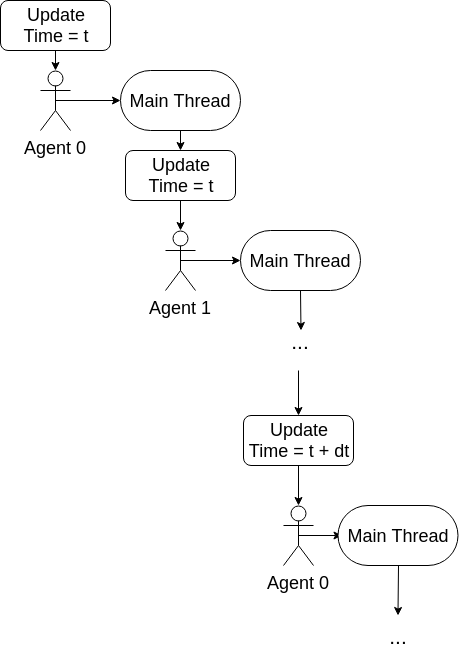
\includegraphics[width=0.3\textwidth, angle=0]{./fig/fpabs/timedriven/sequential.png}
	\caption{Control flow in the Sequential Strategy.}
	\label{fig:strategy_seq}
\end{figure}

\subsection{Parallel Strategy}
This strategy has a globally synchronized time-flow and in each time-step iterates through all the agents and updates them in parallel. Messages sent and changes to the environment made by agents are visible in the next global step. We can think about this strategy in a way that all agents make their moves at the same time.  If one wants to change the environment in a way that it would be visible to other agents this is regarded as a systematic error in this strategy. First it is not logical because all actions are meant to happen at the same time and also it would implicitly induce an ordering, violating the \textit{happens at the same time} idea. 
It does not make a difference if the agents are really executed in parallel or just sequentially - due to the isolation of information, this has the same effect. Also it will make no difference if we iterate over the agents sequentially or randomly, the outcome has to be the same: the strategy is event-ordering invariant as all events and updates happen \textit{virtually at the same time}. This is the strategy used for the implementation of the agent-based SIR model, see below. See Figure \ref{fig:strategy_par} for a visualisation of the control flow in this strategy.

\begin{figure}[H]
	\centering
	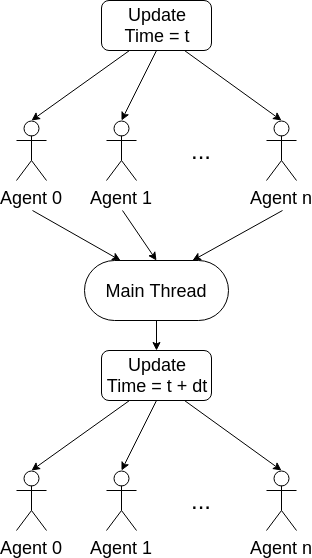
\includegraphics[width=0.3\textwidth, angle=0]{./fig/fpabs/timedriven/parallel.png}
	\caption{Control flow in the Parallel Strategy.}
	\label{fig:strategy_par}
\end{figure}

\subsection{Concurrent Strategy}
This strategy has a globally synchronized time-flow but in each time-step all the agents are updated in parallel with messages sent and changes to the environment are visible immediately. So this strategy can be understood as a more general form of the \textit{parallel strategy}: all agents run at the same time but act concurrently. It is important to realize that, when running agents in parallel, which are able to see actions by others immediately, this is the very definition of concurrency: parallel execution with mutual read/write access to shared data. Of course this shared data-access needs to be synchronized which in turn will introduce event-orderings in the execution of the agents. At this point we have a source of inherent non-determinism: although when one ignores any hardware-model of concurrency, at some point we need arbitration to decide which agent gets access first to a shared resource arriving at non-deterministic solutions. This has the very important consequence that repeated runs with the same configuration of the agents and the model may lead to different results. This strategy will become important in the subsequent chapter on concurrency in ABS where we explain the use of Software Transactional Memory. See Figure \ref{fig:strategy_conc} for a visualisation of the control flow in this strategy.

\begin{figure}[H]
	\centering
	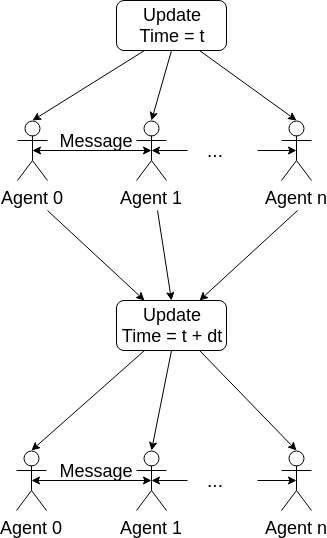
\includegraphics[width=0.3\textwidth, angle=0]{./fig/fpabs/timedriven/concurrent.png}
	\caption{Control flow in the Concurrent Strategy.}
	\label{fig:strategy_conc}
\end{figure}

\subsection{Actor Strategy}
This strategy has no globally synchronized time-flow but all the agents run concurrently in parallel, with their own local time-flow. The messages and changes to the environment are visible as soon as the data arrive at the local agents - this can be immediately when running locally on a multi-processor or with a significant delay when running in a cluster over a network. Obviously this is also a non-deterministic strategy and repeated runs with the same agent- and model-configuration may (and will) lead to different results. It is of most importance to note that information and also time in this strategy is always local to an agent as each agent progresses in its own speed through the simulation. In this case one needs to explicitly \textit{observe} an agent when one wants to e.g. visualize it. This observation is then only valid for this current point in time, local to the observer but not to the agent itself, which may have changed immediately after the observation. This implies that we need to sample our agents with observations when wanting to visualize them, which would inherently lead to well known sampling issues. A solution would be to invert the problem and create an observer-agent which is known to all agents where each agent sends a \textit{'I have changed'} message with the necessary information to the observer if it has changed its internal state. This also does not guarantee that the observations will really reflect the actual state the agent is in but is a remedy against the notorious sampling. The concept of Actors was proposed by \cite{hewitt_universal_1973} for which \cite{greif_semantics_1975} and \cite{clinger_foundations_1981} developed semantics of different kinds. These works were very influential in the development of the concepts of agents and and can be regarded as foundational basics for ABS.  See Figure \ref{fig:strategy_act} for a visualisation of the control flow in this strategy.

\begin{figure}[H]
	\centering
	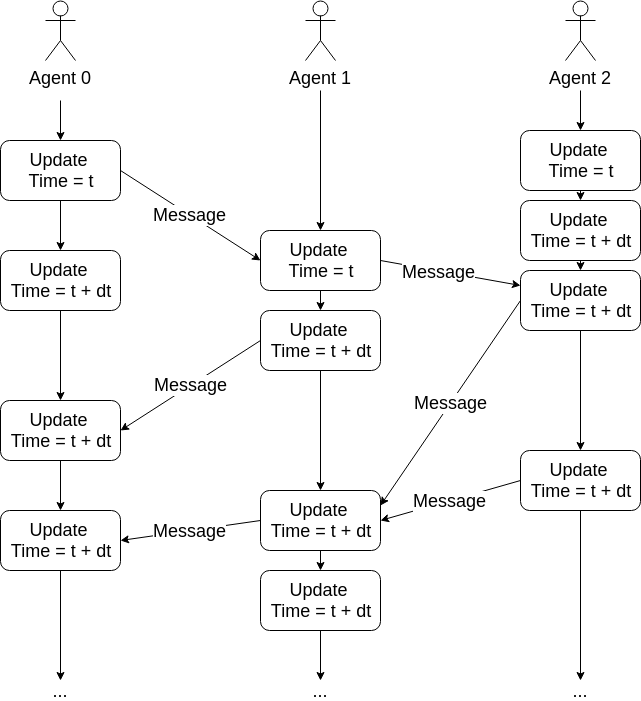
\includegraphics[width=0.3\textwidth, angle=0]{./fig/fpabs/timedriven/actor.png}
	\caption{Control flow in the Actor Strategy.}
	\label{fig:strategy_act}
\end{figure}